% !TeX spellcheck = ru_RU
%pdflatex, utf8
\documentclass[unicode, 10pt, a5paper, oneside]{article}

% Установка полей страницы
%\usepackage{anysize}
%\marginsize{0.3cm}{0.3cm}{0.3cm}{0.3cm}
\usepackage[a5paper, margin=0.3cm, bindingoffset=0cm]{geometry}

% Поддержка русского языка
\usepackage[T2A]{fontenc}		% Корректная кодировка шрифта при использовании cm-super
\usepackage[utf8]{inputenc}		% Кодировка ввода
\usepackage[russian]{babel}		% Словарь расстановки переносов
%\usepackage{cmap}				% Перекодировка символов в pdf при использовании обычного cm

% Всякие математические фишки
\usepackage{amsmath}
\usepackage{amsfonts}
\usepackage{amssymb}

% Изменение цвета, работа с графикой
\usepackage{color}
\usepackage[pdftex]{graphicx}
\graphicspath{{images/}}

% Команда для вставки ссылок \url{URL}
\usepackage[hyphens]{url}
\urlstyle{rm}					% Стиль шрифта ссылок: с засечками

% Кликабельные ссылки внутри документа
\usepackage[unicode]{hyperref}

% Включает отступ у первого абзаца в разделе
\usepackage{indentfirst}

% Настрйока стиля списков
\usepackage{enumitem}
\setlist{noitemsep, leftmargin=*, labelindent=\parindent, topsep=0pt, parsep=0pt, partopsep=0pt}

\setlist[itemize,1]{label=$\diamond$}
\setlist[itemize,2]{label=\textendash}
\setlist[itemize,3]{label=$\star$}

\renewcommand{\alph}[1]{\asbuk{#1}} % Костыль для кирилической нумерации вместо латинской
\setlist[enumerate,1]{label=\arabic*)}
\setlist[enumerate,2]{label=\alph*)}
\setlist[enumerate,3]{label=(\arabic*)}


\usepackage{textcomp}			% Команды для вставки разных символов (градусы, проценты, итд)
\usepackage{float}				% Размещение плавающих объектов там где они созданы (X)
\usepackage{wrapfig}			% Обтекаемые текстом рисунки

% Подписи у флоатов
\setlength{\intextsep}{0pt} % Отстут вокруг плавающих окружений
\usepackage{caption}
\captionsetup{parskip=0pt}
\captionsetup[figure]{labelsep=period,justification=centering,singlelinecheck=false,textfont=small,labelfont=small,aboveskip=2pt,belowskip=0pt}

% Изменение формата заголовков разделов
\usepackage{titlesec}
\titleformat{\section}{\newpage\small\bfseries}{\thesection. }{0pt}{}{}
\titlespacing*{\section}{0pt}{0pt}{0pt}

\titleformat{\subsection}{\small\bfseries}{\thesubsection. }{0pt}{}{}
\titlespacing*{\subsection}{0pt}{0pt}{0pt}

\usepackage{array}				% Позволяет объявить свои типы колонок
\usepackage{calc}				% Математика, исп-ся для расчёта ширины колонки
\usepackage{longtable}			% Длинные таблицы

% Минимальный отступ в таблицах
\setlength{\tabcolsep}{1.5mm}

% Новые типы колонок. Ширина задётся как доля от linewidth
\newcolumntype{L}[1]{p{#1\linewidth-2\tabcolsep-2\arrayrulewidth}}
\newcolumntype{C}[1]{>{\centering}p{#1\linewidth-2\tabcolsep-2\arrayrulewidth}}
\newcolumntype{R}[1]{>{\raggedleft}p{#1\linewidth-2\tabcolsep-2\arrayrulewidth}}
\newcolumntype{U}[2]{p{#1\linewidth-(#2)}}

% Стараться не оставлять одиноких строк в начале и конце абзаца
\clubpenalty=1000
\widowpenalty=1000

% Расстановка отступов и переносов
\emergencystretch=2.5em			% Максимальный промежуток между словами
\tolerance=2000
\frenchspacing


\begin{document}

\setcounter{section}{50}

% Вопрос 51 --------------------------------------------------------
\section{Теорема Котельникова (теорема отсчетов). Квазидетерминированные сигналы.}

В теории и технике сигналов широко используется теорема Котельникова (теорема отсчетов): если наивысшая частота в спектре функции $s(t)$ меньше чем $f_m$ , то функция $s(t)$ полностью определяется последовательностью значений в моменты, отстоящие друг от друга не более чем на $1/2 f_m$ секунд.

В соответствии с этой теоремой сигнал s(t), ограниченный по спектру наивысшей частотой $\omega_m = 2\pi f_m$, можно представить рядом:
\begin{displaymath}
S(t) = \sum_{i=1}^{n}S(kt) \cdot \frac{\sin \omega (t-\frac{n}{2 f_{max}}) }{\omega (t-\frac{n}{2 f_{max}})}
\end{displaymath}
 
где $1/2f_m=\Delta t$ --- обозначает интервал между двумя отсчетными точками на оси времени;

а $s(n/2f_m)=s(n\Delta t)$ --- выборки функции $s(t)$ в момент времени $t=n\Delta t$.

В реальных условиях $f_\text{дискр} = 2f_{max} \cdot k \cdot n \cdot m$

Где $k$ --- коэффициент запаса (1...6);

$n$ --- количество разрядов;

$m$ --- количество каналов.\\

\underline{Квазидетерминированные сигналы.}

Квазидетерминированные модели --- модели, в которых значение одного или нескольких параметров априорно неизвестно.

При описании квазидетерминированных сигналов широко используют понятие элементарного сигнала. 
К элементарным относятся: постоянный сигнал, единичный импульс и синусоидальный сигнал.
\begin{enumerate}
\item Постоянный сигнал представляется соотношением $x = A$, где $A = const$. Единственным параметром постоянного сигнала является значение $A$.
\item Единичный импульс описывается математической моделью вида $x=d(t-t_u)$,
где $d(t-t_u)$ --- дельта-функция, принимающая значение 0 при $t \neq t_\text{и}$ и бесконечность при $t=t_\text{и}$.
\item Гармонический сигнал описывается моделью вида: 
\begin{displaymath}
x(t)= A\cos (\omega t+\varphi)=A\cos (\frac{2\pi}{T} t+\varphi)
\end{displaymath}

и имеет три параметра: амплитуду $A$, частоту $\omega$ (или период $T$) и начальную фазу $\varphi$.

Периодические сигналы могут быть представлены путём разложения их в ряд Фурье:
\begin{displaymath}
x(t)= \frac{A_0}{2} \sum_{k=1}^{\infty} A_k\cos (k \frac{2\pi}{T} t-\varphi_k)
\end{displaymath}

т.е. ряд представлен элементарными гармоническими сигналами.
\item Последовательность прямоугольных импульсов. Для периодических импульсных сигналов определяют производный параметр --- скважность импульсов: $q=T/t_\text{и}$.
\end{enumerate}

% Вопрос 52 --------------------------------------------------------
\section{Преобразование измерительных сигналов. Виды модуляций.}

Передача информации с помощью тех или иных физических процессов осуществляется путем определенного изменения значений их параметров. Подобные операции называются модуляцией. При модуляции мгновенное значение первичного измерительного сигнала управляет одним или несколькими (сложная модуляция) параметрами вспомогательного сигнала, называемого несущим. В качестве несущего сигнала в измерительной технике используют:
\begin{enumerate}
\item постоянный сигнал $z(t) = x_m$ ,
\item гармонический сигнал $z(t) = x_m \cos (\omega t + \varphi)$,
\item периодическую последовательность импульсов.
\end{enumerate}

В соответствии с выбором носителя и информативного параметра различают следующие виды модуляции:
\begin{itemize}
\item ПМ --- прямая модуляция, обеспечиваемая изменением значения постоянного сигнала; 
\item AM --- амплитудная --- $a(t)=A(t)\cos(\omega_0t+\varphi_0)$;
\item УМ --- угловая модуляция. Включает в себя:
	\begin{itemize}
	\item ЧМ --- частотная --- $a(t)=A\cos(\omega(t)t+\varphi_0)$;  
	\item ФМ --- фазовая --- $a(t)=A\cos(\omega_0t+\varphi(t))$; 
	\end{itemize} 
\item АИМ --- амплитудно-импульсная;
\item ВИМ --- время-импульсная. Включает в себя:
	\begin{itemize}
	\item ЧИМ --- частотно-импульсная;
	\item ШИМ --- широтно-импульсная;
	\item ФИМ --- фазоимпульсная модуляция --- вид импульсной модуляции, при которой изменяемым во времени параметром является положение импульсов относительно их исходных (немодулированных) позиций, совпадающих с тактовыми импульсами. 
	\end{itemize}
\item СИМ --- счетно-импульсная;
\item КИМ --- кодоимпульсная модуляции, обеспечиваемые воздействием на соответствующий параметр периодической последовательности импульсных сигналов, используемых в качестве несущих.
\end{itemize}

Модулированное колебание имеет спектр, структура которого зависит как от спектра передаваемого сообщения, так и от вида модуляции. Основным параметром амплитудно-модулированного колебания является глубина модуляции. Отношение $M=\Delta A_m/A_0$ называется коэффициентом модуляции.

\begin{figure}[H]
\centering
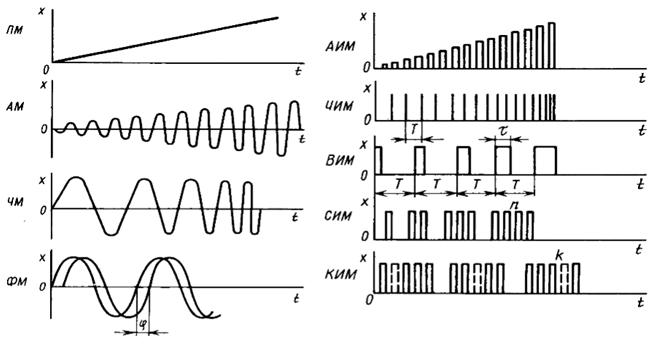
\includegraphics[width=0.7\textwidth]{52.jpg}
\caption{Виды модуляции}
\end{figure}

% Вопрос 53 --------------------------------------------------------
\section{Цифровые частотомеры.}

Цифровые частотомеры являются многофункциональными приборами, в зависимости от режима их работы можно проводить измерение не только частоты, но и интервалов времени (периода следования периодических сигналов). Принцип измерения частоты гармонического сигнала цифровым методом поясняет структурная схема цифрового частотомера в режиме измерения частоты и временные диаграммы к его работе.
\begin{figure}[H]
\centering
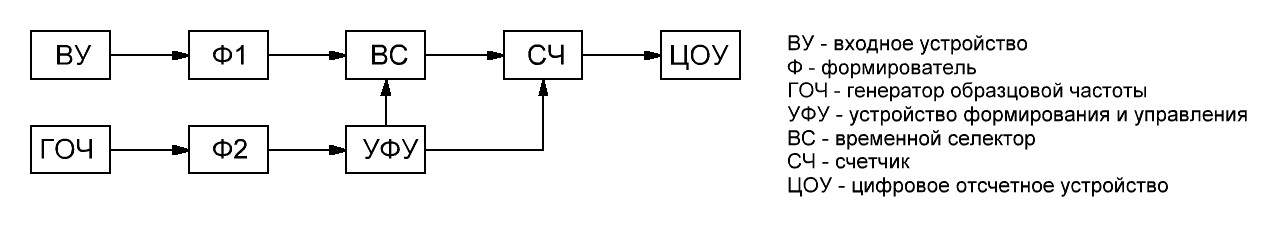
\includegraphics[width=0.9\textwidth]{53.jpg}
\caption{Структурная схема цифрового частотомера}
\end{figure}

Исследуемый гармонический сигнал, имеющий частоту $f_x$ , подается на входное устройство (ВУ), усиливающее или ослабляющее его до значения, требуемого для работы последующего устройства частотомера. Формирователь Ф1 состоит из усилителя-ограничителя и компаратора (триггера Шмитта).

Счетные импульсы поступают на один из входов временного селектора (ВС), на второй вход которого от устройства формирования и управления (УФУ) подаётся строб-импульс прямоугольной формы и калиброванной длительности. Временной селектор открывается строб-импульсом  и в течение его длительности пропускает группу (пакет) импульсов на вход счетчика (СЧ). В результате на счетчик поступает пакет из $N_X$ импульсов.

\begin{figure}[H]
\centering
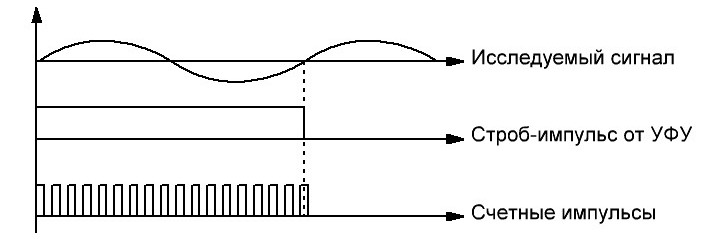
\includegraphics[width=0.65\textwidth]{53_dia.jpg}
\caption{Временная диаграмма работы цифрового частотомера}
\end{figure}

Для формирования строб-импульса на устройство УФУ поступают короткие импульсы с периодом $T_0$ от схемы, включающей генератор образцовой частоты (ГОЧ) и второй формирователь импульсов (Ф2), аналогичный формирователю Ф1. В составе ГОЧ имеется кварцевый генератор образцовой частоты и декадный делитель частоты. Период импульсов на выходе формирователя Ф2 и длительность строб-импульсов равны периоду сигнала на выходе делителя частоты.

Счетчик подсчитывает $N_X$ импульсов и выдает соответствующий (двоичный) код в цифровое отсчетное устройство (ЦОУ). Циклический режим работы частотомера задаётся УФУ, при этом перед началом каждого измерения УФУ сбрасывает показания счетчика в ноль. Максимальная ошибка --- 1 интервал тактового сигнала, то есть определяющим звеном частотомера является опорный генератор.

Для измерения ВЧ сигналов возможен режим работы, при котором заполнение интервала происходит импульсами самого входного сигнала, а ГОЧ формирует точный интервал.

% Вопрос 54 --------------------------------------------------------
\section{Цифровые фазометры.}

Цифровые фазометры предназначены для измерений углов поворота, снятия фазочастотных характеристик различных звеньев. Цифровые фазометры можно разделить на две группы: для измерения мгновенного значения сдвига фаз и для измерения среднего значения сдвига фаз. Сдвиг по фазе $\varphi$ между двумя напряжениями $u_1 (t)$ и $u_2 (t)$ легко преобразуется во временной интервал $\tau$.
Поэтому схема цифрового фазометра отличается от схемы ЦИП для измерения временных интервалов двумя формирователями Ф1 и Ф2, формирующими старт- и стоп-импульсы в момент перехода кривых напряжений $u_1 (t)$ и $u_2 (t)$ через нуль, и блоком выделения временного интервала БВВИ (см. рис.).

\begin{figure}[H]
\centering
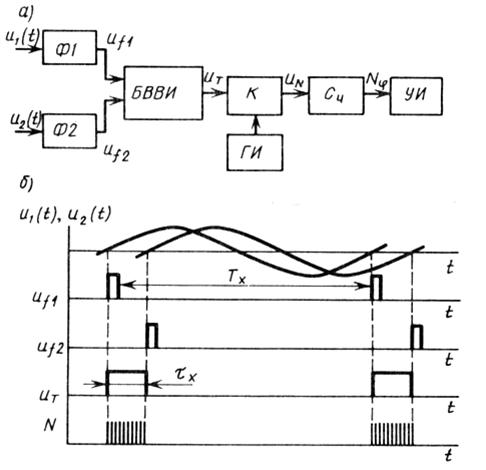
\includegraphics[width=0.65\textwidth]{54.jpg}
\caption{Цифровой фазометр: а --- структурная схема; б --- временная диаграмма; (БВВИ --- блок выделения временных интервалов; Ф --- формирователь; К --- ключ; ГИ --- генератор импульсов; Сч --- счетчик; УИ --- устройство индикации)}
\end{figure}

В соответствии со структурной схемой, количество импульсов сигнала $U_N (t)$ образцовой частоты $f_0$ с ГИ, поступившее за время $\tau_x$ в счетчик Сч, будет равно $N_X = \tau_x f_0$. Отсюда получаем:
\begin{displaymath}
\varphi_x = \frac{2\pi \tau_x N_X}{f_0}
\end{displaymath}

При измерении фазового сдвига необходимо либо обеспечить постоянство частот измеряемых сигналов $f_1$ и $f_2$, либо обеспечить постоянство отношения $f_x/f_0$.

% Вопрос 55 --------------------------------------------------------
\section{Цифровые вольтметры временного преобразования.}

Цифровые вольтметры (ЦВ) временного преобразования реализуются по методу развертывающего преобразования и могут быть неинтегрирующими и интегрирующими (ИЦВ).

\underline{Неинтегрирующие ЦВ} предназначены для измерения мгновенных значений входного напряжения. Эти вольтметры не защищены от действия помех и не обеспечивают высокой чувствительности и разрешающей способности. Здесь значение измеряемого напряжения их предварительно преобразуется в интервал времени $T_x$, который кодируется методом последовательного счета. В ЦВР преобразование $U_x$ в $T_x$ производится посредством сравнения $U_x$ с линейно изменяющимся напряжением $U_p$, формируемым генератором пилообразного напряжения (ГПН).

\begin{figure}[H]
\centering
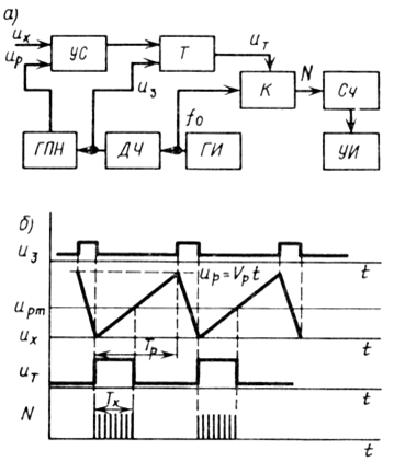
\includegraphics[width=0.5\textwidth]{55_1.jpg}
\caption{Цифровой вольтметр развертывающего временного преобразования}
\end{figure}

Импульсы запуска $U_\text{з}$, вырабатываемые генератором импульса ГИ и делителем частоты ДЧ, устанавливают триггер Т в единичное состояние и запускают ГПН, который формирует напряжение развертки $U_p=\upsilon_p t$, где $\upsilon_p =U_{pm}/T$ --- скорость нарастания пилообразного напряжения; $U_{pm}$ --- максимальное значение напряжения развертки; $T$ --- время развертки. Обычно ГПН представляет собой интегратор, подключаемый на заданное время к источнику постоянного опорного напряжения. В момент равенства $U_x$ и $U_p$ устройство сравнения УС вырабатывает импульс, возвращающий триггер Т в нулевое состояние. Триггер Т формирует импульс длительностью $T_x=U_x/U_p$ в течение которой открыт ключ К и импульсы образцовой частоты поступают в счетчик Сч. Количество импульсов, накапливаемых в Сч, равно: 

\begin{displaymath}
N = T_x f_0 = \frac{U_x f_0}{\upsilon_p}
\end{displaymath}

\underline{Интегрирующие цифровые вольтметры} получили наибольшее распространение среди цифровых вольтметров. Главное достоинство их --- высокая помехозащищенность.

Как известно, самой распространенной помехой является переменное напряжение с частотой промышленной сети.
Интегрирование входного напряжения, т. е. усреднение за некоторый фиксированный интервал времени, позволяет получить результат (теоретически) без влияния помехи. Метод интегрирования нашел свое развитие в ИЦВ двухтактного интегрирования, в которых происходит сравнение интегралов измеряемого и образцового напряжений.

Работа ИЦВ инициируется поступлением импульса запуска от устройства управления и триггер Т1 открывает ключ К2, разрешая тем самым прохождение на интегратор И измеряемого напряжения $U_x$. Одновременно открывается ключ К3 и импульсы с частотой $f_0$ с ГИ поступают на вход ДЧ. При выбранном коэффициенте деления К0 через время $t_0 = t_2 --- t_1$ на выходе ДЧ появляется импульс управления триггера Т2 и Т1, который инвертирует их состояния. Тем самым закрывается ключ К2, заканчивая интегрирование измеряемого напряжения $U_x$, и открывается ключ К1, подключающий на вход И опорное напряжение ${U_\text{оп}}$, полярность которого противоположна $U_x$.

\begin{figure}[H]
\centering
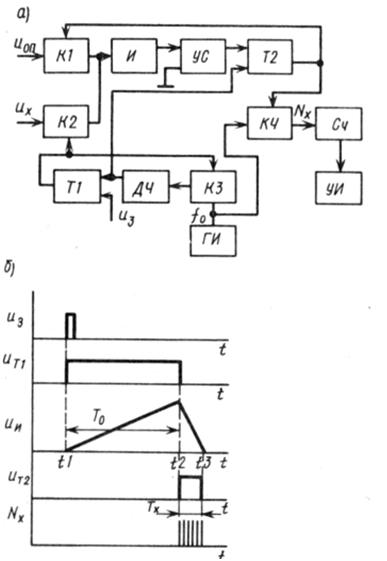
\includegraphics[width=0.5\textwidth]{55_2.jpg}
\caption{Интегрирующий цифровой вольтметр (К --- ключ; Т --- триггер; И --- интегратор; УС --- устройство сравнения; Сч --- счетчик; ГИ --- генератор импульсов; УИ --- устройство индикации).}
\end{figure}

В момент времени $t_3$, когда напряжение равно 0, срабатывает устройство сравнения УС, триггер Т2 возвращается в исходное состояние, ключ К1 закрывается и интегрирование заканчивается. Импульс T2 с длительностью $T_x$ открывает счетчик Сч. Количество импульсов при этом пропорционально среднему значению измеряемого напряжения.

Результат измерения не зависит от значения постоянной времени интегрирования интегратора и частоты $f_0$.
ИЦВ двухтактного интегрирования имеют значительно меньшую погрешность измерения, чем ЦВ развертывающего временного преобразования. Интегрирующие ЦВ используются в ИИС в качестве прецизионных АЦП.

% Вопрос 56 --------------------------------------------------------
\section{Микропроцессорные цифровые измерительные преобразователи.}

Появление первых микропроцессоров (МП) в интегральном исполнении и дальнейший быстрый их прогресс и удешевление коренным образом изменили подходы к разработке многофункциональных ЦИП. Применение МП в измерительной технике позволяет резко повысить точность приборов, значительно расширить их возможности, повысить надежность, решать задачи, которые ранее вообще не рассматривались.

Основные функции, возлагаемые на МП в ЦИП:
\begin{enumerate}
\item измерение --- управление АЦ-преобразованием: линеаризация функции преобразования; автоматический выбор пределов измерения; выбор каналов и типов измерения; компенсация помех; исключение систематических погрешностей;
\item обработка --- накопление массивов измерительной информации; косвенное измерение; статистическая и другие виды обработки; сжатие данных; адаптация к входному сигналу;
\item управление --- прием управляющих воздействий оператора; настройка прибора на режим работы; контроль за действиями оператора с возможностью коррекции его ошибок; выдача справочной информации; сигнализация в экстремальных ситуациях;
\item отображение --- управление работой СОИ; хранение результатов предыдущих измерений; отображение текстовой информации большого объема; отображение графической информации; вспомогательная и сервисная информация (время, дата и т.п.);
\item интерфейсные функции --- управление интерфейсом; работа в комплексе с другими ЦИП;
\item тестовые функции --- самотестирование; калибровка измерительных каналов.
\end{enumerate}

В ряде случаев для ЦИП создают многопроцессорную систему управления, в которой осуществляется специализация функций процессоров: процессор ввода-вывода, процессор управления, процессор обработки и т.д.

Применение в измерительной технике МП породило новый класс цифровых программируемых многоканальных измерительных приборов, получивших за рубежом наименование логгеров (регистраторы данных). Типовой логгер построен на концепции шинной организации и по блочно-модульному типу. Здесь все элементы измерительной системы рассматриваются как внешние устройства (ВУ) для МП или микроЭВМ. Логгеры могут содержать до 100 измерительных каналов, опрашиваемых синхронно или асинхронно, причем частота опроса может изменяться в широких пределах. Встроенный МП управляет прибором согласно заданной программе. В большинстве современных логгеров программа управления хранится на дисках.

\begin{figure}[H]
\centering
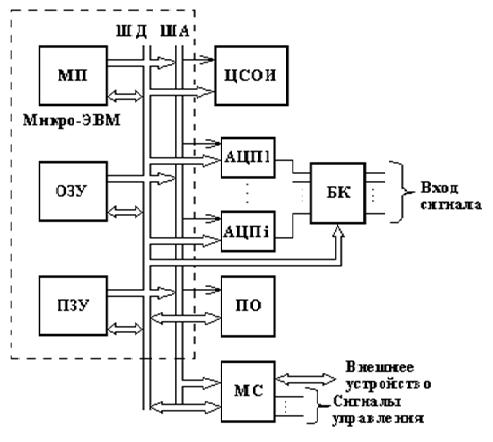
\includegraphics[width=0.55\textwidth]{56.jpg}
\caption{Обобщенная структурная схема регистратора данных}
\end{figure}

% Вопрос 57 --------------------------------------------------------
\section{Резистивные датчики (реостатные, пьезорезистивные).}

Измерительный параметр --- омическое сопротивление. К резистивным датчикам с механическим перемещением относят реостатные, пьезорезисторы, тензорезисторы.
\begin{enumerate}
\item \underline{Реостатные датчики} --- преобразуют измеряемую величину в омическое сопротивление. Реостатные датчики представляют собой переменное сопротивление специальной конструкции, движок которого под действием входной величины $x$ меняет свое положение.  Наиболее часто такие датчики применяются для измерения перемещений, для измерения уровня жидкости и пр. На первом этапе измеряемая величина преобразуется в перемещение движка переменного резистора. Изготавливаются из манганина, константана, вольфрама. Требования к материалам: минимальный температурный коэффициент, устойчивость к механическим воздействиям. Движок должен обеспечивать хороший электрический контакт. Движок --- сплав платины и лития.

Резистивные преобразователи применяются в системах, где прилагаемое усилие не менее $10^{-2}$ Н, величина перемещения не менее 2 мм, а частота питания не более 5 Гц. Для изменения формы кривой зависимости сопротивления датчика от перемещения движка меняют плотность намотки или форму каркаса.

\item \underline{Тензорезисторы} --- используются для исследования механических напряжений. Они изготавливаются из проволоки, фольги и полупроводниковых пластинок. Их принцип действия основан на изменении электрического сопротивления под действием механической деформации. Тензорезистивный преобразователь состоит из базы, на которую наклеена проволока диаметром 0,02 --- 0,03 мм зигзагообразной формы. К концам проволоки приварены выводные провода. Сверху провода нанесен слой лака. Датчик наклеен на исследуемую поверхность и вместе с ней деформируется, преобразуя механическое напряжение в изменение омического сопротивления. Для преобразования приращения сопротивления могут быть использованы как мостовые схемы, так и схемы с делителями напряжения.

Фольговые и проволочные тензорезисторы имеют коэффициент тензочувствительности от 0,5 до 40, в то время как полупроводниковые --- от 40 до 200.
\end{enumerate}

% Вопрос 58 --------------------------------------------------------
\section{Электромагнитные датчики (индуктивные, трансформаторные, магнитоупругие).}

\underline{Индуктивные датчики}. Принцип действия индуктивных датчиков основан на изменении индуктивности L или взаимоиндуктивности обмотки с сердечником вследствие изменения магнитного сопротивления магнитной цепи датчика, в которую входит сердечник. Индуктивные датчики относятся к классу параметрических. Измеряемое механическое перемещение на входе датчика вызывает изменение параметров магнитной и электрической цепей его, что в свою очередь вызывает изменение выходной величины --- электрического тока I. С помощью индуктивных датчиков можно контролировать механические перемещения, температуру, свойства магнитных материалов. Индуктивные датчики используются на относительно низких частотах (до 3000-5000 Гц), так как на высоких частотах резко растут потери в стали на перемагничивание и вихревые токи.

\underline{Трансформаторные датчики}. Наиболее удобны для практических применений, так как выходной параметр их --- ЭДС. Применяют для повышения точности измерений. При отсутствии перемещения сердечника в обмотках трансформатора индуцируются одинаковые ЭДС, сумма которых ввиду их встречного соединения равна нулю. При появлении перемещения в одной половине магнитной цепи за счет уменьшения воздушного зазора возрастает магнитный поток, увеличивается наводимая ЭДС во вторичной обмотке. Аналогично уменьшается ЭДС во второй половине датчика ввиду увеличения воздушного зазора. Возникающая результирующая (суммарная) ЭДС пропорциональна значению перемещения.

\begin{figure}[H]
\centering
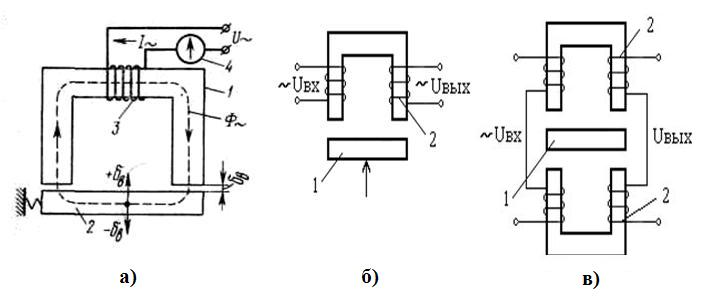
\includegraphics[width=0.7\textwidth]{58.jpg}
\caption{Индуктивный датчик (а), одноэлементный (б) и дифференциальный (в) трансформаторные датчики}
\end{figure}

\underline{Магнитоупругие датчики}. Среди датчиков индуктивного типа особое место занимают магнитоупругие,  принцип действия которых основан на изменении магнитной проницаемости сердечника под действием механической силы Q.

Магнитоупругий датчик представляет собой магнитопровод  прямоугольной формы с четырьмя симметрично расположенными отверстия-ми, в которых размещены две обмотки, причем плоскости этих обмоток взаимно перпендикулярны. Одна обмотка питается током переменного напряжения, а вторая является измерительной. При полной симметрии магнитопровода и изотропности материала индуктивная связь между обмотками отсутствует, следовательно, ЭДС обмотки при отсутствии механических напряжений в материале магнитопровода равна нулю.

При воздействии на магнитопровод механического усилия Q нарушается изотропность материала вследствие изменения магнитных свойств последнего под действием упругих напряжений и, как следствие этого, при этом часть потока питающей обмотки пересекает витки измерительной обмотки, в результате чего в последней наводится ЭДС, возрастающая с увеличением действующего на магнитопровод усилия.
Достоинства: простота конструкции, высокая надежность, возможность измерения больших сил ($10^5 - 10^6$ Н). Недостатки: невысокая точность: погрешность 1-4 %.

% Вопрос 59 --------------------------------------------------------
\section{Пьезоэлектрические датчики.}

Некоторые диэлектрики при воздействии на них механического усилия подвергаются электрической поляризации, что представляет собой явление прямого пьезоэффекта. Обратный пьезоэффект характеризуется тем, что диэлектрический материал под воздействием электрического поля подвергается механической деформации. При этом пьезоэффект обладает знакочувствительностью, т. е. при изменении направления механического напряжения изменяется полярность электрических зарядов и при изменении полярности электрического поля меняется направление механической деформации диэлектрика.

К материалам, обладающим пьезоэффектом, можно отнести кварц, сегнетову соль и другие кристаллические вещества, а также искусственные керамики: титанат бария, титанат свинца, цирконат свинца и др.

Пьезоэлектрические датчики относятся к датчикам генераторного типа. Обычно для увеличения чувствительности пьезодатчика применяют две или несколько пластинок, соединенных параллельно; при этом заряды одноименно заряжающихся плоскостей должны складываться.

\begin{figure}[H]
\centering
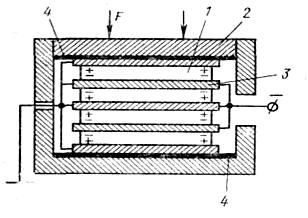
\includegraphics[width=0.45\textwidth]{59.jpg}
\caption{Пьезоэлектрический датчик}
\end{figure}

Мощность, развиваемая пьезоэлементом, чрезвычайно мала, ввиду этого измерительная цепь датчика тщательно экранируется от помех и наводок.

При измерении статических сил возникающий электрический заряд утекает через сопротивление измерительной цепи, следовательно, исключается возможность их регистрации. Поэтому практически пьезоэлектрические датчики применяются для регистрации лишь динамических сил. Частотный диапазон измерений составляет $10^5-10^6$  Гц.
В измерительной цепи пьезодатчиков обычно используется усилитель с входным сопротивлением не менее $10^{13}$ Ом с малой входной емкостью. Дифференцирующий характер пьезоэлектрических  преобразователей позволяет на их базе построить датчики виброускорений --- акселерометры.

% Вопрос 60 --------------------------------------------------------
\section{Тепловые датчики (термопары, термометры сопротивления).}

Для измерения температуры последняя преобразуется в промежуточную величину, например в ЭДС, электрическое сопротивление и другие величины. Для регистрации больших температур используется оптический метод. Из всех существующих методов измерения температуры наиболее широко применяются термоэлектрические.

Термоэлектрический эффект заключается в том, что при соединении двух проводов из разных материалов (термопара) и создании разности температур между точкой соединения и точками свободных концов возникает ЭДС, пропорциональная разности температур. Значение термоЭДС зависит от материалов термопары и колеблется в пределах от долей до сотен милливольт на 100 °С. Характеристика термоэлектрических преобразователей, как правило, нелинейная и в значительной степени зависит от наличия примесей, механической и термической обработки материалов термопары.

Каждая термопара снабжается градуировочной характеристикой. Градуировка термопар осуществляется при температуре свободных концов, равной нулю; при температуре, отличной от нуля, возникает дополнительная погрешность.

При градуировке термопар для исключения погрешности от непостоянства внутреннего сопротивления прибора последний градуируется совместно с датчиком.

\begin{table}[H]
\caption{Термопары}
\centering\small
\begin{tabular}{|c|c|c|c|c|c|}
\hline
Наименование	& Обозн.	& Материалы				& Диапазон		& Макс. $t^\circ$	& Чувствит., мВ/$^\circ$C \\ \hline
ТПП 			& ПП-1		& Pt(40\%), Pt-Ro		& -60...+1300	& 1600				& 1,4 \\ \hline
ТПР 			& ПР-30/6	& Pt+30\%Ro, Pt+6\%Ro	& -200...+1100	& 1400				& 10 \\ \hline
ТХА 			& ХА		& Cr-Al					& -50...+1000	& 1300				& 40 \\ \hline
ТХК 			& ПП-1		& Cr-Co					& -50...+600	& 800				& 800 \\ \hline
\end{tabular}
\end{table}

Термометры-сопротивления имеют две основные разновидности: термосопротивления с платиновым (ТСП) и медным (ТСМ) чувствительными элементами. Современные платиновые терморезистивные датчики температуры имеют вид спирали, помещенной в канавках двух- или четырехканального керамического каркаса и уплотненной порошкообразной окисью алюминия. Такая конструкция позволяет использовать преобразователь как в защитной арматуре, так и без нее.

Медный терморезистивный чувствительный элемент представляет собой бескорпусную обмотку из медной изолированной проволоки, покрытую сверху фторопластовой пленкой. Для обеспечения необходимой прочности обмотку помещают в тонкостенную металлическую гильзу, которую засыпают керамическим порошком и герметизируют.

Характеристика терморезисторов наиболее близка к линейной.

\begin{table}[H]
\caption{Термосопротивления}
\centering
\begin{tabular}{|c|c|c|c|}
\hline
Тип	& $R_\text{ном}$& Группа ТС	& Диапазон, $^\circ$C\\
	& при $0^\circ$C&			&				\\ 
\hline
ТСП & 1				& 1П		& -50...+1100	\\ 
	& 5				& 5П		& -100...+1100	\\ 
	& 10			& 10П		& -200...+1000	\\ 
	& 50			& 50П		& -200...+1000	\\ 
	& 100			& 100П		& -260...+1000	\\ 
\hline
ТСМ	& 10			& 10М		& -50...+100	\\ 
	& 50			& 50М		& -50...+200	\\ 
	& 100			& 100М		& -200...+200	\\ 
\hline
\end{tabular}
\end{table}



\begin{table}[H]
\caption{Соответствие классов точности и допусков}
\centering
\begin{tabular}{|c|c|c|}
\hline
Тип	& Класс точности& Допуск, \%\\
\hline
ТСП & I				& 0,05		\\ 
	& II			& 0,1		\\ 
	& III			& 0,2		\\ 
	& IV			& 0,4		\\ 
	& V				& 0,8		\\ 
\hline
ТСМ	& II			& 0,1		\\ 
	& III			& 0,2		\\
	& IV			& 0,5		\\ 
	& V				& 1			\\ 
\hline
\end{tabular}
\end{table}

\end{document}